% Created 2023-10-30 Mon 18:01
% Intended LaTeX compiler: pdflatex
\documentclass[12pt, a4paper]{article}
\usepackage[utf8]{inputenc}
\usepackage[T1]{fontenc}
\usepackage{graphicx}
\usepackage{longtable}
\usepackage{wrapfig}
\usepackage{rotating}
\usepackage[normalem]{ulem}
\usepackage{amsmath}
\usepackage{amssymb}
\usepackage{capt-of}
\usepackage{hyperref}
\usepackage{placeins}
\usepackage{gensymb}
\usepackage[letterpaper]{geometry}
\geometry{top=1.0in, bottom=1.0in, left=1.0in, right=1.0in}
\usepackage{rotating}
\usepackage{graphicx}
\usepackage{pgfplots}
\usepackage{filecontents}
\usepackage{tikz}
\usepackage{fancyhdr}
\usepackage{enumitem}
\pagestyle{fancy}
\lhead{}
\chead{}
\rhead{Johnson \thepage}
\lfoot{}
\cfoot{}
\rfoot{}
\renewcommand{\headrulewidth}{0pt}
\renewcommand{\footrulewidth}{0pt}
\setlength\headsep{0.333in}
\newcommand{\bibent}{\noindent \hangindent 40pt}
\newenvironment{workscited}{\newpage \begin{center} Works Cited \end{center}}{\newpage }
\graphicspath{ {./attachments/} }
\author{Christian}
\date{\today}
\title{}
\hypersetup{
 pdfauthor={Christian},
 pdftitle={},
 pdfkeywords={},
 pdfsubject={},
 pdfcreator={Emacs 28.2.50 (Org mode 9.7-pre)}, 
 pdflang={English}}
\begin{document}

\begin{document}
\begin{flushleft}
Christian Johnson\\
\vspace{2mm}Dr. Paul Crilly\\
\vspace{2mm}Antennas and Propogation\\
\vspace{2mm}October 28 2023\\
\vspace{4mm}\begin{center}
Lab 7 Report
\end{center}
\vspace{1mm}\setlength{\parindent}{0.5in}

\begin{abstract}
This study aimed to investigate the behavior and bandwidth characteristics of various antennas, including a copper pipe dipole, 0.025 and 1/8 inch dipoles, bowtie, and helical antennas. The primary goal was to gain a deeper understanding for how these antennas perform across different frequency ranges. Observations revealed that the copper pipe dipole displayed a SWR below 2 between 113.7 MHz and 131.12 MHz, without noticeable SWR graph flattening. The 0.024-inch dipole showed SWR values below 2 from 111.5 MHz to 124.5 MHz, transitioning to traveling wave behavior at around 144.5 MHz. The 1/8-inch dipole exhibited SWR below 2 from 111.5 MHz to 116.75 MHz, with flattening observed shortly after 118 MHz. The bowtie antenna achieved SWR below 2 from 114.75 to 143.35 MHz, with a consistent standing wave profile. The helical antenna didn't dip below 2 MHz but displayed signs of flattening around 1.328 GHz.Our findings offered insights into the diverse characteristics of these antennas, showcasing their adaptability to varying frequency requirements. Additionally, we calculated the bandwidth for each antenna, revealing significant distinctions in their ability to cover a range of frequencies efficiently. This knowledge equips us to make informed decisions in practical applications, enhancing antenna selection and optimization for specific purposes. 
\end{abstract}
\section*{Procedures}
\label{sec:org81a489f}
The purpose of this lab was to determine the bandwidth for a series of antennas. We used a 0.024 inch wire dipole, a 1/8 of an inch wire dipole, a 1.2 inch copper pipe dipole, a bowtie antenna, and a helical antenna. Each of these antennas had different operating frequencies, with the three dipoles and the bowtie antenna at 120MHz and the helical at 900 MHz. In order to find the bandwidth for each antenna at their lowest frequency, we will use an Agilent Frequency analyzer to determine the range where SWR is less than or equal to 2. We can check the SWR graph to see what frequency it starts to flatten, in order to determine when the antenna starts to act like a traveling wave antenna. Using the data from this experiment, we are able to determine the bandwidth - information that is extremely useful to know when working with antennas. 
\section*{Results}
\label{sec:org3aa898f}
In order to understand the bandwidth and SWR behavior for this group of antennas, we analyzed their SWR over a range of frequencies. The copper pipe dipole demonstrated an SWR below 2 within the frequency range of 113.7 MHz and 131.12 MHz. Despite this pattern, we did not observe any noticeable flattening in the SWR graph. The 0.024 inch dipole displayed SWR values below 2 from 111.5 MHz to 124.5 MHz, and began to behave like a traveling wave antenna around 144.5 MHz. The 1/8 inch dipole showcased an SWR below 2 from 111.5 MHz to 116.75 MHz, beginning to flatten just after 118 MHz. The Bowtie antenna dipped below an SWR of 2 from 114.75 to 143.35 MHz. We did not notice the SWR graph for the Bowtie antenna begin to flatten, which would indicate that it never stops acting like a standing wave antenna. The helical antenna never actually dipped below 2 MHz, but we did notice it begin to flatten around 1.328 GHz. These observations help us to understand the characteristics of each type of antenna, allowing us to better understand their behavior under certain conditions. Using each antenna's upper and lower bounds, we are able to find their bandwidth. In general, bandwidth can be represented by the equation \(B_p=2*\frac{f_{u}-f_{l}}{f_{u}+f_{l}}*100\%\), where \(f_u\) and \(f_l\) are the upper and lower bounds respectively. The copper pipe dipole exhibits a bandwidth of 14.23, 11.01 for the 0.024 inch dipole, 4.6 for the 1/8 inch dipole, and 22.16 for the bowtie antenna. Since we were unable to find a frequency range for the helical antenna, we were unable to properly calculate a bandwidth.
\section*{Conclusions}
\label{sec:orga3f091d}
In this investigation, our aim was to gain insight into the behavior of different antennas, particularly regarding their SWR characteristics and overall performance. The antennas in question included the copper pipe dipole, the 0.024-inch wire dipole, the 1/8-inch wire dipole, the bowtie antenna, and the helical antenna, each designed for varying operating frequencies.

Our exploration of these antennas unveiled valuable information about their unique behaviors. We found distinctions in how SWR values fluctuated across their respective frequency ranges. These observations provided a understanding of how each antenna type reacts under different conditions.

By examining the SWR behavior, we managed to identify important transitions, such as when some antennas began to exhibit traveling wave characteristics. These findings contribute to a broader understanding of antenna versatility and how they adapt to varying frequency requirements.


\newpage
\begin{center}
Appendices
\end{center}
\begin{figure}[htb]
\centering
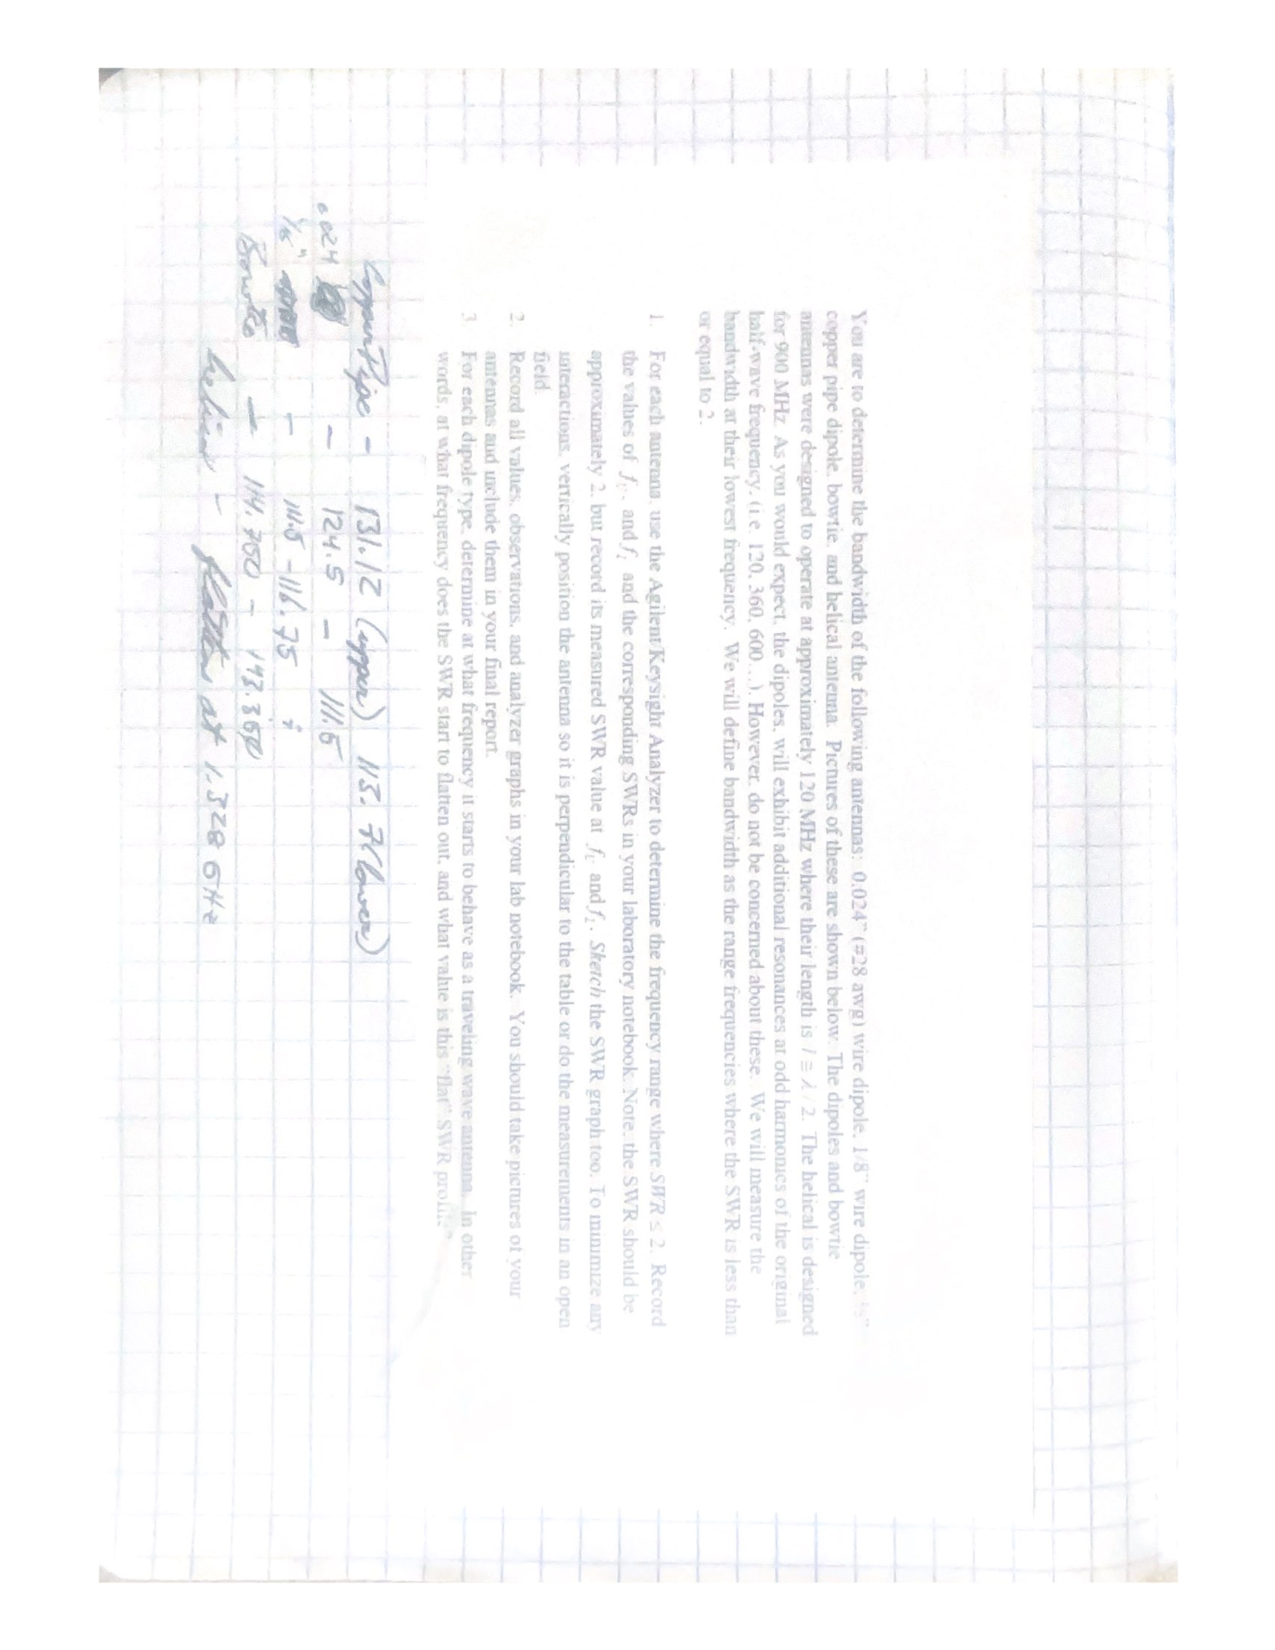
\includegraphics[angle=90,page=1,width=0.5\textwidth]{Lab7.pdf}
\caption{Notebook Page 1}
\end{figure}
\begin{figure}[htb]
\centering
\includegraphics[angle=90,page=2,width=0.5\textwidth]{Lab7.pdf}
\caption{Notebook Page 2}
\end{figure}
\newpage
\newpage

\pagebreak
\begin{center}
Lab Questions
\end{center}
\vspace{2mm}
\begin{enumerate}[label=\textbf{\arabic*.}]
\item How did the thickness affect the bandwidth?
Thicker elements, like the copper pipe, exhibited a wider bandwidth, whereas thinner elements had narrower bandwidths.
\item How does the bowtie antenna's bandwidth compare to that of the thin wire antennas?
The bowtie demonstrated a wider bandwidth than any of the thin wire antennas.
\item Theoretically, why do the copper pipe and bowtie antennas have more/less bandwidth than the thin wires?
The copper pipe and bowtie antennas have unique geometries that widen their frequency range. The triangular elements help to increase the bandwidth compared to the straight elements in wire dipoles. These triangular elements effectively help ensure that the antenna's impedance characteristics are stable over a wide frequency range.
\item Compare the helical antennas bandwidth to the wire dipoles.
Since we were unable to properly calculate the helical antennas bandwidth, we are unable to effectively compare it. However, in theory, the helical antenna's long length can help it operate over a wide range of frequencies since, when an antenna is significantly longer than the wavelength, it begins to act like a travelling wave antenna.
\item Indicate when SWR flattened and its value.
We did not observe flattening in the copper pipes SWR graph. The 0.024 inch dipole began to flatten around 144.5 MHz, with an SWR of about 2.6. The 1/8 inch dipole began to flatten around 118 MHz with an SWR of about 2.3. We did not note flattening in the bowtie graph either, and the helical antenna flattened around 1.328 GHz. Since the SWR graph for the helical antenna fluctuated more than the others, it was difficuly to accurately record an SWR measurement, but the flat section had an approximate SWR of about 3.4.
\item Why would travelling wave antennas not be used on VHF and UHF bands?
Travelling wave antennas are typically rather large. At lower frequencies this size is manageable, but becomes less so as frequency increases. Travelling wave antennas are also more directional than is usually suited for VHF and UHF, since these frequencies often involve multiple directions at the same time. Travelling wave antennas are also better suited for narrower bandwidths. VHF and UHF cover a relatively wide range of frequencies, making it more challenging to maintain consistant performance across the entire band. 
\end{enumerate}

\end{document}
\end{document}